\documentclass[border=3pt]{standalone}
\usepackage{mathptmx}
\usepackage{tikz}
\usetikzlibrary{positioning,arrows.meta,fit,calc,decorations.pathreplacing,backgrounds}
\definecolor{cblue}{HTML}{2A78D6}\definecolor{corange}{HTML}{EB6834}\definecolor{caqua}{HTML}{1BAF7A}
\definecolor{ink}{HTML}{0B0B0B}\definecolor{ink2}{HTML}{52514E}\definecolor{muted}{HTML}{8A8984}\definecolor{fillg}{HTML}{F3F2EE}
\definecolor{fblue}{HTML}{DBE8F8}\definecolor{forange}{HTML}{FDE3D8}
\begin{document}
\hyphenpenalty=10000 \exhyphenpenalty=10000 \frenchspacing
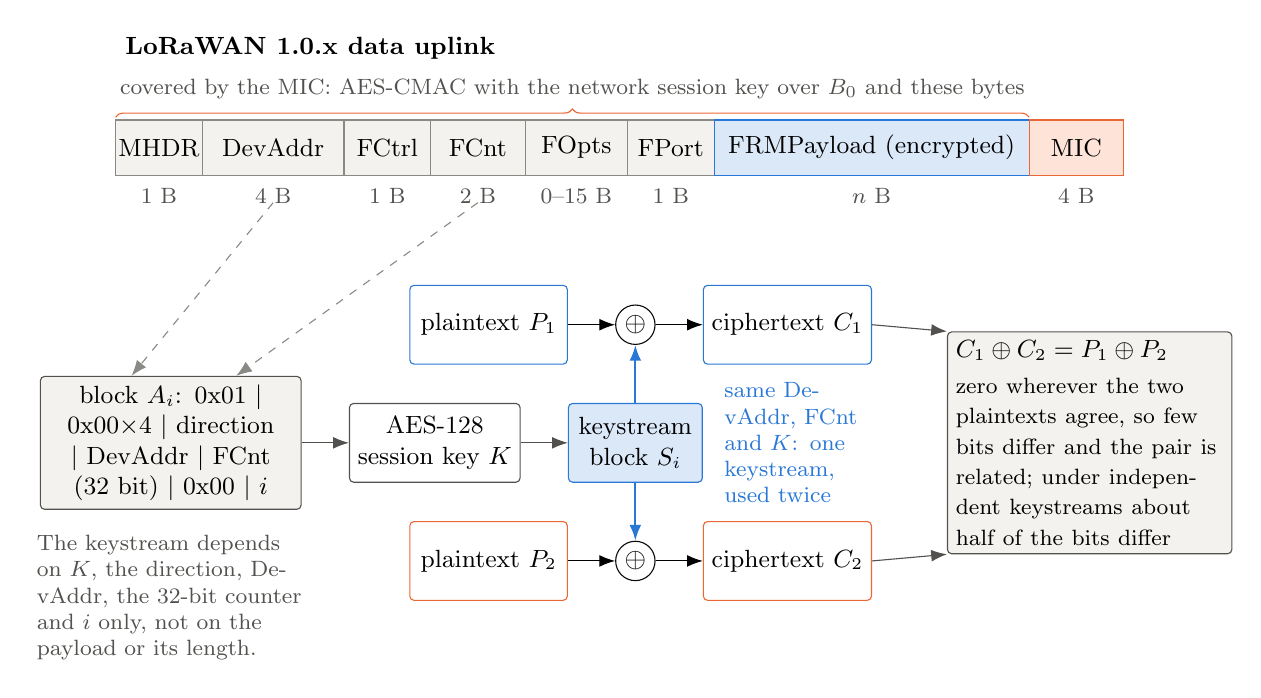
\begin{tikzpicture}[font=\small, >={Latex[length=2mm]},
  fld/.style={draw=muted, fill=fillg, minimum height=7mm, inner sep=1pt, outer sep=0pt},
  blk/.style={draw=ink2, rounded corners=1.5pt, align=center, minimum height=10mm, inner sep=3pt},
  sz/.style={font=\footnotesize, text=ink2},
  note/.style={font=\footnotesize, text=ink2, align=left}]
% ---- the frame
\node[fld, minimum width=11mm] (mhdr) at (0,0) {MHDR};
\node[fld, minimum width=18mm, right=0mm of mhdr] (addr) {DevAddr};
\node[fld, minimum width=11mm, right=0mm of addr] (fctrl) {FCtrl};
\node[fld, minimum width=12mm, right=0mm of fctrl] (fcnt) {FCnt};
\node[fld, minimum width=13mm, right=0mm of fcnt] (fopts) {FOpts};
\node[fld, minimum width=11mm, right=0mm of fopts] (fport) {FPort};
\node[fld, draw=cblue, fill=fblue, minimum width=40mm, right=0mm of fport] (pay) {FRMPayload (encrypted)};
\node[fld, draw=corange, fill=forange, minimum width=12mm, right=0mm of pay] (mic) {MIC};
\foreach \n/\t in {mhdr/1, addr/4, fctrl/1, fcnt/2, fopts/0--15, fport/1, pay/$n$, mic/4}
  \node[sz, below=0.4mm of \n] {\t\ B};
\draw[decorate, decoration={brace, amplitude=3pt, raise=1pt}, draw=corange] (mhdr.north west) -- (pay.north east)
  node[midway, above=4pt, note] {covered by the MIC: AES-CMAC with the network session key over $B_0$ and these bytes};
\node[font=\small\bfseries, anchor=south west] at ($(mhdr.north west)+(0,6.5mm)$) {LoRaWAN 1.0.x data uplink};
% ---- keystream row (y = 0 of this part), with the two frames above and below the keystream block
\coordinate (o) at ($(mhdr.south west)+(66mm,-34mm)$);
\node[blk, draw=cblue, fill=fblue, minimum width=17mm] (ks) at (o) {keystream\\ block $S_i$};
\node[blk, left=6mm of ks, minimum width=20mm] (aes) {AES-128\\ session key $K$};
\node[blk, fill=fillg, left=6mm of aes, text width=31mm] (ai)
  {block $A_i$: 0x01 $|$ 0x00${\times}$4 $|$ direction $|$ DevAddr $|$ FCnt (32 bit) $|$ 0x00 $|$ $i$};
\draw[->, ink2] (ai) -- (aes); \draw[->, ink2] (aes) -- (ks);
\draw[->, muted, dashed] ($(addr.south)+(0,-3.5mm)$) -- ($(ai.north west)!0.35!(ai.north east)$);
\draw[->, muted, dashed] ($(fcnt.south)+(0,-3.5mm)$) -- ($(ai.north west)!0.75!(ai.north east)$);
\node[note, below=2mm of ai, text width=34mm] {The keystream depends on $K$, the direction, DevAddr, the 32-bit counter and $i$ only, not on the payload or its length.};
\node[circle, draw=ink, inner sep=0pt, minimum size=5mm, font=\normalsize] (x1) at ($(ks)+(0,15mm)$) {$\oplus$};
\node[circle, draw=ink, inner sep=0pt, minimum size=5mm, font=\normalsize] (x2) at ($(ks)+(0,-15mm)$) {$\oplus$};
\node[blk, draw=cblue, left=6mm of x1, minimum width=20mm] (p1) {plaintext $P_1$};
\node[blk, draw=corange, left=6mm of x2, minimum width=20mm] (p2) {plaintext $P_2$};
\node[blk, draw=cblue, right=6mm of x1, minimum width=20mm] (c1) {ciphertext $C_1$};
\node[blk, draw=corange, right=6mm of x2, minimum width=20mm] (c2) {ciphertext $C_2$};
\draw[->] (p1) -- (x1); \draw[->] (x1) -- (c1); \draw[->] (p2) -- (x2); \draw[->] (x2) -- (c2);
\draw[->, cblue, thick] (ks.north) -- (x1.south); \draw[->, cblue, thick] (ks.south) -- (x2.north);
\node[note, text=cblue, right=1.5mm of ks, text width=19mm] {same DevAddr, FCnt and $K$: one keystream, used twice};
\node[blk, fill=fillg, anchor=west, text width=34mm, align=left] (eq) at ($(ks.east)+(31mm,0)$)
  {$C_1 \oplus C_2 = P_1 \oplus P_2$\\[2pt]{\footnotesize zero wherever the two plaintexts agree, so few bits differ and the pair is related; under independent keystreams about half of the bits differ}};
\draw[->, ink2] (c1.east) -- (eq.north west); \draw[->, ink2] (c2.east) -- (eq.south west);
\end{tikzpicture}
\end{document}
